\documentclass[tikz]{standalone}
\usepackage{tikz}

\usetikzlibrary{positioning}
\usetikzlibrary{fit}
\usetikzlibrary{shapes}
\usetikzlibrary{arrows}

\tikzstyle{X} = [circle,fill=white,draw=black]
% Observed node
\tikzstyle{Y} = [X,fill=gray!25]
\tikzset{>={triangle 45}}

\begin{document}

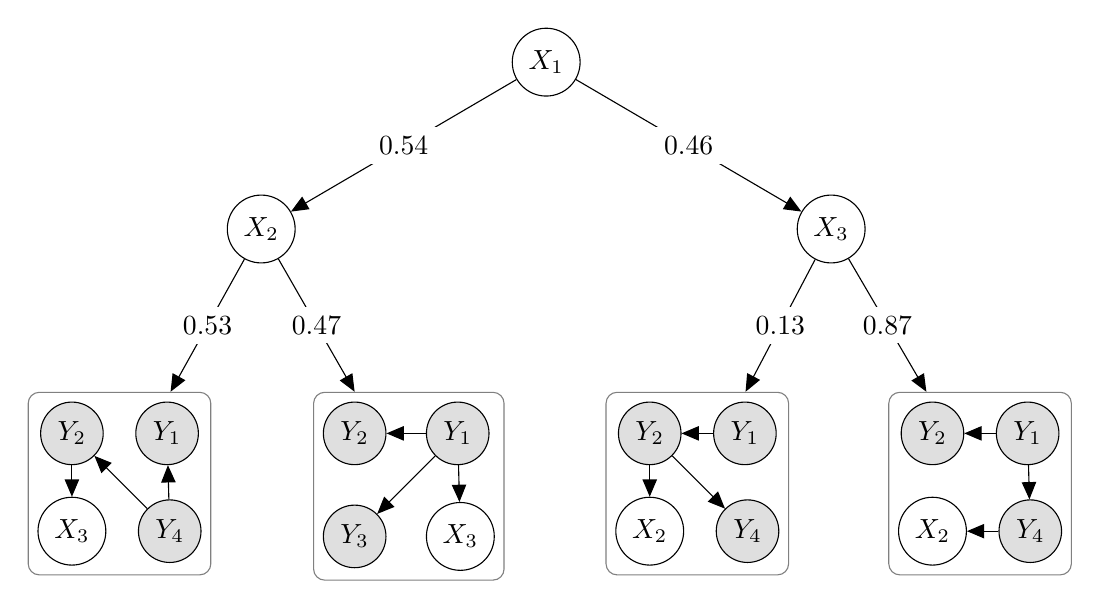
\begin{tikzpicture}
  \node [X] (n1) {$X_1$};    
  \node [X,below left=1.5cm and 3cm of n1] (n2) {$X_2$};    
  \node [X,below right=1.5cm and 3cm of n1] (n3) {$X_3$};    
  % \node [X,below left=2.5cm of n3] (n4) {$X_1$};    
  % \node [X,below right=2.5cm of n1] (n5) {$X_4$};    
  % \node [X,below right=2.5cm of n5] (n6) {$X_3$};
  \draw [->] (n1) -- (n2) node [midway,fill=white] {0.54};
  \draw [->] (n1) -- (n3) node [midway,fill=white] {0.46};

  \node [Y,below right=2cm and 1.9cm of n2] (n7) {$Y_1$};
  \node [Y,left=0.5cm of n7] (n8) {$Y_2$};
  \node [Y,below=0.5 of n8] (n9) {$Y_3$};
  \node [X,right=0.5 of n9] (n10) {$X_3$};
  % \node [X,below=0.5 of n10] (n101) {$X_1$};
  \node [draw=gray,rectangle,rounded corners,fit=(n7) (n8) (n9) (n10)] (r1) {};
  \draw [->] (n7) -- (n8) ;
  \draw [->] (n7) -- (n9);
  \draw [->] (n7) -- (n10);
  \draw [->] (n2) -- (r1) node [midway,fill=white] {0.47};
  
  

  
  %\draw [->] (n1) -- (n5) node [midway,fill=white] {0.46};

  \node [Y,below right=2cm and 1.9cm of n3] (n11) {$Y_1$};
  \node [Y,left=0.4cm of n11] (n12) {$Y_2$};
  \node [X,below=0.4 of n12] (n13) {$X_2$};
  \node [Y,right=0.4 of n13] (n14) {$Y_4$};
  \node [draw=gray,rectangle,rounded corners,fit=(n11) (n12) (n13)
  (n14)] (r2) {};
  \draw [->] (n3) -- (r2) node [midway,fill=white] {0.87};
  \draw [->] (n11) -- (n12);
  \draw [->] (n14) -- (n13);
  \draw [->] (n11) -- (n14);

   

  \node [Y,below left=2cm and .5cm of n3] (n15) {$Y_1$};
  \node [Y,left=0.4cm of n15] (n16) {$Y_2$};
  \node [X,below=0.4 of n16] (n17) {$X_2$};
  \node [Y,right=0.4 of n17] (n18) {$Y_4$};
  \node [draw=gray,rectangle,rounded corners,fit=(n15) (n16) (n17)
  (n18)] (r3) {};
  \draw [->] (n16) -- (n17);
  \draw [->] (n16) -- (n18);
  \draw [->] (n15) -- (n16);
  \draw [->] (n3) -- (r3) node [midway,fill=white] {0.13};

  \node [Y,below left=2cm and .6cm of n2] (n19) {$Y_1$};
  \node [Y,left=0.4cm of n19] (n20) {$Y_2$};
  \node [X,below=0.4 of n20] (n21) {$X_3$};
  \node [Y,right=0.4 of n21] (n22) {$Y_4$};
  \node [draw=gray,rectangle,rounded corners,fit=(n19) (n20) (n21)
  (n22)] (r4) {};
  \draw [->] (n20) -- (n21);
  \draw [->] (n22) -- (n20);
  \draw [->] (n22) -- (n19);
  \draw [->] (n2) -- (r4) node [midway,fill=white] {0.53};
  
  

\end{tikzpicture}
\end{document}

%%% Local Variables:
%%% mode: latex
%%% TeX-master: t
%%% End:
